\documentclass[hidelinks]{article}
    \usepackage[utf8]{inputenc}
    
    \usepackage{pgfplots}
    \pgfplotsset{compat=1.6}
    \usepackage{graphicx}
    \usepackage{mathptmx}
    \usepackage{wrapfig}
    \usepackage{color}
    \usepackage{lscape}
    \usepackage{amsmath}
    
    \usepackage[none]{hyphenat}
    \usepackage{times}
    \usepackage[T1]{fontenc} % Use 8-bit encoding that has 256 glyphs
    \linespread{1.05} % Line spacing - Palatino needs more space between lines
    \usepackage{microtype} % Slightly tweak font spacing for aesthetics
    \usepackage[left=25mm, right=25mm,top=25mm, bottom=32mm,columnsep=20pt]{geometry} % Document margins
    \usepackage[hang, small,labelfont=bf,up,textfont=it,up]{caption} % Custom captions under/above floats in tables or figures
    \usepackage{booktabs} % Horizontal rules in tables
    \usepackage{float} % Required for tables and figures in the multi-column environment - they need to be placed in specific locations with the [H] (e.g. \begin{table}[H])
    \usepackage{hyperref} % For hyperlinks in the PDF
    \usepackage{paralist} % Used for the compactitem environment which makes bullet points with less space between them
    \setlength\parindent{5mm}
    
    \usepackage{abstract}
    \renewcommand{\abstractname}{}
    \renewcommand{\absleftindent}{5mm}
    \renewcommand{\absrightindent}{5mm}
    
    \usepackage{sectsty}
    \sectionfont{\fontsize{14}{1em}\selectfont}
    
    \usepackage{fancyhdr}
    \pagestyle{fancy}
    \fancyhead{}
    \renewcommand{\headrulewidth}{0.5pt}
    \renewcommand{\footrulewidth}{0.5pt}
    % \fancyfoot{}
    % \rhead{TF coil model in PROCESS - Version 1.0}

    \usepackage{tikz}
    \usetikzlibrary{shapes}
    \usetikzlibrary{arrows}
    \usetikzlibrary{patterns}

    \usepackage{caption}

    \definecolor{plotColour1}{HTML}{6699CC}
    \definecolor{plotColour2}{HTML}{CC3333}
    \definecolor{plotColour3}{HTML}{C0C0C0}
    \definecolor{plotColour4}{HTML}{FFCC00}
    \definecolor{plotColour5}{HTML}{66CCCC}
    \definecolor{midnight_blue}{HTML}{2c3e50}
    \definecolor{belize_hole}{HTML}{2980b9}
    \definecolor{gray}{HTML}{BAC1B8}
    \definecolor{cadetblue}{HTML}{58A4B0}
    \definecolor{turq}{HTML}{0C7C59}
    \definecolor{gunmetal}{HTML}{2B303A}
    \definecolor{vermillion}{HTML}{D64933}
    \definecolor{quicksilver}{HTML}{9DA9A0}
    \definecolor{weldon_blue}{HTML}{7A9E9F}
    \definecolor{purple_navy}{HTML}{3D5A80}
    
    \usepackage[numbers]{natbib}
    %\usepackage{cite}
    \setlength{\bibsep}{2.0mm}
    \numberwithin{equation}{section}
    
    \title{Toroidal Field Coil Model in PROCESS}
    \author{James Morris and sebastien Kahn}
    \date{January 2020}

    \newenvironment{noi}{\noindent}
    
    \begin{document}
    
    \maketitle
    
    \tableofcontents
    
    \clearpage
    
    \section{Introduction}
    
    The PROCESS systems code performs an integrated and self-consistent treatment 
    of the physics, engineering, economic, safety and environmental characteristics 
    of a fusion power plant \cite{kovari2014}. PROCESS takes an input file with 
    instructions detailing the parameters that can vary and a list of consistency 
    equations to use. The user is able to set fixed values for certain parameters.\\
    
    \noi This document details the superconducting (SC) Toroidal Field (TF) coil module 
    in PROCESS. The model calculates the geometry of the winding pack and coil, the 
    allowable current densities, the maximum field and many other physical quantities 
    related to the coils. These properties are described in \S 3.\\

    \noi Another part of the module determines the stresses exerted on the TF coil given 
    a set of inputs such as the current and structural make-up of the coil. PROCESS 
    will have limits to the allowable stress in the input file (or by default). If 
    the calculated stresses are above the limits then PROCESS will attempt to minimise 
    the stresses until they are within the allowable range. The stress model is 
    detailed in \S 5.

    \section{Coil Geometry}
    \label{sec:geom}

    This section outlines the geometry used in the TF model. Figure 
    \ref{fig: geom-1}  shows the overall geometry of the TF coil inboard leg excluding 
    dimensions of the internal make-up of the coil (e.g. winding pack). Where 
    \texttt{r\_tf\_inleg\_in} is the coil inner radii, \texttt{rtfcin} the coil centre radii, 
    \texttt{r\_tf\_inleg\_out} the coil outer radii, \texttt{tfcth} is the total thickness of 
    the inboard TF coil and \texttt{theta\_coil} is the half toroidal angular extent of the coil.
        
    \begin{figure}[!b]
     \begin{center}
      \begin{tikzpicture}[scale=1.4]rc (-30:30:50mm);
        \draw[thick] (7.45,2)--(4.6,2.5);
        \draw[thick] (7.45,5)--(4.6,4.3);
        \draw[thick] (4.6,2.5)--(4.6,4.3);
        \draw[thick] (7.45,5)--(7.45,2);
        \tikzstyle{block} = [draw,fill=blue!10,minimum size=1em]
        \tikzstyle{cloud} = [draw, circle]
        \filldraw[fill=black] (6.1,3.4) circle (0.05cm);
        \draw (6.15,3.6) node {rtfcin};
        \filldraw[fill=black] (7.45,3.4) circle (0.05cm);
        \draw (7.15,3.6) node {r\_tf\_inleg\_out};
        \filldraw[fill=black] (4.6,3.4) circle (0.05cm);
        \draw (4.95,3.6) node {r\_tf\_inleg\_in};  
        \draw[thick, dashed] (0,3.4)--(8,3.4);
        \draw[thick, dashed] (0.8,3.4)--(4.55,4.275);
        \draw[thick] [<->,>=stealth] (4.8,2.7)--(7.3,2.7);
        \draw (6.1,2.9) node {tfcth};
        \draw (2.71,3.6) node {theta\_coil/2};
       \end{tikzpicture}
    \end{center}
    \caption{Cross-sectional geometry of TF coil inner leg.} \label{fig: geom-1}
    \end{figure}

    \section{Winding Pack}

    \noi The toroidal angular extent of a single TF coil inner leg is:

    \begin{equation}\label{eq: theta_coil}
    \text{theta\_coil} = \frac{\pi}{\text{n\_tf}} 
    \end{equation}

    \noi where \emph{n\_tf} is the number of TF coils (seen in figure \ref{fig: geom-1}). 
    Assuming an annular geometry, the area of the coil inboard leg is given by  

    \begin{equation}\label{eq: tfareain}
    \text{tfareain} = \pi (\text{r\_tf\_inleg\_out}^2 - \text{r\_tf\_inleg\_in}^2) 
    \end{equation}

    \noi After defining the dimensions of the inboard leg PROCESS calculates 
    the internal dimensions of the coil. As shown in figure 2, the radial thickness 
    of the TF coil winding pack is:

    \begin{equation}\label{eq:dr_tf_wp}
    \text{dr\_tf\_wp} = \text{tfcth} - \text{casthi} - \text{thkcas} - 2\times \text{tinstf} 
    - 2\times \text{tfinsgap}
    \end{equation}

    \subsection{Winding pack with non-integer turns}

    \noi For the winding pack with non-integer turns PROCESS models a winding pack 
    that has two thicknesses, one for each half of the winding pack (see figure 
    \ref{fig: winding-pack-non-integer}). The thicknesses are:

    \begin{equation}\label{eq: wwp1}
    \text{wwp1} = 2(\text{radwp}\times \tan(\text{theta\_coil}) - \text{casths} - \text{tinstf} 
    - \text{tfinsgap}); \hspace{0.3cm} r > \text{radwp}
    \end{equation}

    \begin{equation}\label{eq: wwp2}
    \text{wwp2} = 2((\text{radwp}-\frac{1}{2}\text{dr\_tf\_wp})\times \tan(\text{theta\_coil}) - 
    \text{casths} - \text{tinstf}); \hspace{0.3cm} r < \text{radwp} 
    \end{equation}

    \noi Where \emph{radwp} is the radial centre of the winding pack (the two sections, 
    \emph{wwp1} and \emph{wwp2}, have the same radial width). Using these thicknesses, and 
    other defined parameters, PROCESS calculates the relative areas of different materials in 
    the coil. The total cross-sectional area of the winding pack is:

    \begin{equation}\label{eq: awptf}
    \text{awptf} = (\frac{1}{2}\text{dr\_tf\_wp})(\text{wwp1}+\text{wwp2}) 
    \end{equation}

    \noi The area of the entire winding pack, the insulation and insertion gap is:

    \begin{equation}\label{eq: awpc}
    \text{awpc} = \frac{1}{2}\text{dr\_tf\_wp}(\text{wwp2} + 2\times \text{tinstf} 
    + 2\times \text{tfinsgap}) + (\frac{1}{2}\text{dr\_tf\_wp} + 2\times \text{tinstf})(\text{wwp1} 
    + 2 \times \text{tinstf} + 2\times \text{tfinsgap})
    \end{equation}

    \noi Using this area one can find the area of the TF inboard leg that 
    is not winding pack or insulation; i.e. the case area. The calculation of the 
    vertical stress on the TF coil uses this area.

    \begin{equation}\label{eq: acasetf}
    \text{acasetf} = \frac{\text{tfareain}}{\text{n\_tf}} - \text{awpc}
    \end{equation}

    \noi Given the relative winding pack areas PROCESS calculates the dimensions of 
    the SC cables. PROCESS defines a single turn then uses the winding pack area to 
    calculate the number of turns in the inner leg. The winding pack current density is:

    \begin{equation}
    j_{wptf} = \text{max}(1.0, \frac{\text{ritfc}}{\text{n\_tf} \times \text{awptf}})
    \end{equation}

    \begin{figure}[t!]
     \begin{center}
      \begin{tikzpicture}[scale=1.0]
            
        % Machine bore
        \draw (0.4,0.5) node [rotate=90] {bore};  
        \draw[dashed] (1.0,-1)--(1.0,1);
        
        % Central solenoid (CS)
        \draw (1.5,0.6) node [rotate=90] {ohcth};
        \draw[dashed] (2.0,-1)--(2.0,1);
        
        % CS pre-compression structure
        \draw (2.5,0.8) node [rotate=90] {precomp};  
        \draw[dashed] (3.0,-1)--(3.0,1);
        
        % Gap between CS precompression and TF coil
        \draw (3.5,0.6) node [rotate=90] {gapoh};  
        
        % mid dashed line
        \draw[dashed] (0,0)--(4.0,0);
        
        % Coil outline
        \filldraw[thick, fill=white!90!black, line width=0.3mm] 
        (4,-2)--(4,2)--(4,2)--(9,3)--(9,3)--(9,-3)--(9,-3)--(4,-2);
        \filldraw[thick, fill=white!90!black, line width=0.1mm] 
        (10,2.5)--(10.25,2.5)--(10.25,2.25)--(10,2.25)--(10,2.5);
        \draw[align=left] (11.0,2.375) node {Steel};  
        
        % Insertion gap
        \filldraw[thick, fill=cadetblue, line width=0.2mm] 
        (6.8,0)--(6.8,2.2)--(7.55,2.2)--(7.55,2.45)--(8.7,2.45)
        --(8.7,-2.45)--(7.55,-2.45)--(7.55,-2.2)--(6.8,-2.2)--(6.8,0);
        \filldraw[thick, fill=cadetblue, line width=0.1mm] 
        (10,1.5)--(10.25,1.5)--(10.25,1.25)--(10,1.25)--(10,1.5);
        \draw (11.70,1.35) node {Insertion Gap};  
        
        % Groundwall insulation
        \filldraw[thick, fill=vermillion, line width=0.2mm]
        (6.9,0)--(6.9,2.1)--(7.65,2.1)--(7.65,2.35)--(8.6,2.35)
        --(8.6,-2.35)--(7.65,-2.35)--(7.65,-2.1)--(6.9,-2.1)--(6.9,0);
        \filldraw[thick, fill=vermillion, line width=0.1mm] 
        (10,0.5)--(10.25,0.5)--(10.25,0.25)--(10,0.25)--(10,0.5);
        \draw (11.8,0.375) node {Groundwall Ins};  
        
        % Winding pack
        \filldraw[thick, fill=quicksilver, line width=0.2mm]
        (7,0)--(7, 2)--(7.75,2)--(7.75,2.25)--(8.5,2.25)--(8.5,-2.25) --(7.75,-2.25)--(7.75,-2)--(7,-2)--(7,0);
        \filldraw[thick, fill=quicksilver, line width=0.1mm] 
        (10,-0.5)--(10.25,-0.5)--(10.25,-0.75)--(10,-0.75)--(10,-0.5);
        \draw (11.7,-0.65) node {Winding Pack};
        
        % labels
        
        % Inboard case
        \draw[dashed] (4.0,-2)--(4.0,-4);
        \draw[dashed] (6.8,-2.25)--(6.8,-4.9);
        \draw [<->,>=stealth] (4.0,-3.5)--(6.8,-3.5);
        \draw (5.4,-3.8) node {thkcas};
        
        % Insertion Gap
        \draw[dashed] (6.9,-2.25)--(6.9,-4.9);
        \draw [->,>=stealth] (6.5,-4.5)--(6.8,-4.5);
        \draw [<-,>=stealth] (6.9,-4.5)--(7.2,-4.5);
        \draw (6.1,-4.8) node {tinsgap};
        
        % Groundwall insulation
        \draw[dashed] (6.9,2.15)--(6.9,5);
        \draw[dashed] (7.0,2.15)--(7.0,5);
        \draw [->,>=stealth] (6.6,4.5)--(6.9,4.5);
        \draw [<-,>=stealth] (7.0,4.5)--(7.3,4.5);
        \draw (6.2,4.2) node {tinstf};
        
        % Winding Pack
        % \draw[dashed] (9.5,-2.5)--(9,2.5);
        \draw [<->,>=stealth] (7.15,2)--(7.15,-2);
        \draw (7.4,0) node [rotate=90] {wwp2};
        
        % \draw[dashed] (8.5,2.25)--(8.5,4);
        \draw [<->,>=stealth] (8.0,-2.25)--(8.0,2.25);
        \draw (8.25,0) node [rotate=90] {wwp1};
        
        % Side casing
        \draw[dashed] (6.8,2.2)--(4.0,2.2);
        \draw[dashed] (6.8,2.55)--(4.0,2.55);
        \draw [->,>=stealth] (4.25,2.85)--(4.25,2.55);
        \draw [<-,>=stealth] (4.25,2.2)--(4.25, 1.9);
        \draw (4.85,2.8) node {casths};
        
        % Plasma facing casing
        \draw[dashed] (8.7,-2.25)--(8.7,-4.9);
        \draw[dashed] (9.0,-2.25)--(9.0,-4.9);
        \draw [->,>=stealth] (8.4,-4.5)--(8.7,-4.5);
        \draw [<-,>=stealth] (9.0,-4.5)--(9.3,-4.5);
        \draw (9.6,-4.8) node {casthi};
               
       \end{tikzpicture}
      \end{center}
     \caption{Diagram of internal make up of TF coil and radial build of 
     components closer to the device centreline for a TF coil with non-integer turns. The 
     relevant PROCESS variable names are shown.} \label{fig: winding-pack-non-integer}
    \end{figure}

    \subsection{Winding pack with integer turns}

    The number of pancakes (\emph{n\_pancake}) and the number of layers (\emph{n\_layer}) 
    for the integer turn model are input by the user. The total number of turns is
    
    \begin{equation}\label{eq: turnstf-int}
        \text{turnstf} = \text{n\_pancake} \times \text{n\_layer}
    \end{equation}

    \noi For the winding pack with integer turns PROCESS models a winding pack 
    that has one thicknesses (see figure \ref{fig: winding-pack-integer}). The winding 
    pack thickness is given as:

    \begin{equation}\label{eq: wwp1-int}
    \text{wwp1} = 2(\text{radwp}\times \tan(\text{theta\_coil}) - \text{casths} - \text{tinstf} 
    - \text{tfinsgap}); \hspace{0.3cm} r > \text{radwp}
    \end{equation}

    \noi The area of the winding pack is

    \begin{equation}\label{eq: awptf-int}
    \text{awptf} = \text{dr\_tf\_wp} \times \text{wwp1}
    \end{equation}

    \noi The area of the entire winding pack, the insulation and insertion gap is:

    \begin{equation}\label{eq: awpc-int}
    \text{awpc} = (\text{dr\_tf\_wp} + 2\times \text{tinstf} + 2\times \text{tfinsgap}) 
    \times (\text{wwp1} + 2\times \text{tinstf} + 2\times \text{tfinsgap})
    \end{equation}

    \noi Using this area one can find the area of the TF inboard leg that 
    is not winding pack or insulation; i.e. the case area. The calculation of the 
    vertical stress on the TF coil uses this area.

    \begin{equation}\label{eq: acasetf-int}
    \text{acasetf} = \frac{\text{tfareain}}{\text{n\_tf}} - \text{awpc}
    \end{equation}

    \noi Given the relative winding pack areas PROCESS calculates the dimensions of 
    the SC cables. PROCESS defines a single turn then uses the winding pack area to 
    calculate the number of turns in the inner leg. The winding pack current density is:

    \begin{equation}
    j_{wptf} = \text{max}(1.0, \frac{\text{ritfc}}{\text{n\_tf} \times \text{awptf}})
    \end{equation}

    \begin{figure}[t!]
        \begin{center}
         \begin{tikzpicture}[scale=1.0]
           
           % Machine bore
           \draw (0.4,0.5) node [rotate=90] {bore};  
           \draw[dashed] (1.0,-1)--(1.0,1);
           
           % Central solenoid (CS)
           \draw (1.5,0.6) node [rotate=90] {ohcth};
           \draw[dashed] (2.0,-1)--(2.0,1);
           
           % CS pre-compression structure
           \draw (2.5,0.8) node [rotate=90] {precomp};  
           \draw[dashed] (3.0,-1)--(3.0,1);
           
           % Gap between CS precompression and TF coil
           \draw (3.5,0.6) node [rotate=90] {gapoh};  
           
           % mid dashed line
           \draw[dashed] (0,0)--(4.0,0);
           
           % Coil outline
           \filldraw[thick, fill=white!90!black, line width=0.3mm] 
           (4,-2)--(4,2)--(4,2)--(9,3)--(9,3)--(9,-3)--(9,-3)--(4,-2);
           \filldraw[thick, fill=white!90!black, line width=0.1mm] 
           (11,2.5)--(11.25,2.5)--(11.25,2.25)--(11,2.25)--(11,2.5);
           \draw[align=left] (12.0,2.375) node {Steel};  
           
           % Insertion gap
           \filldraw[thick, fill=cadetblue, line width=0.2mm] 
           (6.8,0)--(6.8,2.2)--(8.7,2.2)--(8.7,-2.2)--(6.8,-2.2)--(6.8,0);
           \filldraw[thick, fill=cadetblue, line width=0.1mm] 
           (11,1.5)--(11.25,1.5)--(11.25,1.25)--(11,1.25)--(11,1.5);
           \draw (12.70,1.35) node {Insertion Gap};  
           
           % Groundwall insulation
           \filldraw[thick, fill=vermillion, line width=0.2mm] 
           (6.9,0)--(6.9,2.1)--(8.6,2.1)--(8.6,-2.1)--(6.9,-2.1)--(6.9,0);
           \filldraw[thick, fill=vermillion, line width=0.1mm] 
           (11,0.5)--(11.25,0.5)--(11.25,0.25)--(11,0.25)--(11,0.5);
           \draw (12.8,0.375) node {Groundwall Ins};  
           
           % % Winding pack
           \filldraw[thick, fill=quicksilver, line width=0.2mm]  
           (7,0)--(7,2)--(8.5,2)--(8.5,-2)--(7,-2)--(7,0);
           \filldraw[thick, fill=quicksilver, line width=0.1mm] 
           (11,-0.5)--(11.25,-0.5)--(11.25,-0.75)--(11,-0.75)--(11,-0.5);
           \draw (12.7,-0.65) node {Winding Pack};
           
           % labels
           
           % Inboard case
           \draw[dashed] (4.0,-2)--(4.0,-4);
           \draw[dashed] (6.8,-2.25)--(6.8,-4.9);
           \draw [<->,>=stealth] (4.0,-3.5)--(6.8,-3.5);
           \draw (5.4,-3.8) node {thkcas};
           
           % Insertion Gap
           \draw[dashed] (6.9,-2.25)--(6.9,-4.9);
           \draw [->,>=stealth] (6.5,-4.5)--(6.8,-4.5);
           \draw [<-,>=stealth] (6.9,-4.5)--(7.2,-4.5);
           \draw (6.1,-4.8) node {tinsgap};
           
           % Groundwall insulation
           \draw[dashed] (6.9,2.15)--(6.9,5);
           \draw[dashed] (7.0,2.15)--(7.0,5);
           \draw [->,>=stealth] (6.6,4.5)--(6.9,4.5);
           \draw [<-,>=stealth] (7.0,4.5)--(7.3,4.5);
           \draw (6.2,4.2) node {tinstf};
           
           % Winding Pack
           \draw[dashed] (8.5,2.25)--(8.5,4);
           \draw [<->,>=stealth] (7.0,3.0)--(8.5,3.0);
           \draw (7.7,4.25) node [rotate=90] {t\_wp\_radial};

           \draw[dashed] (8.5,2)--(10,2);
           \draw[dashed] (8.5,-2)--(10,-2);
           \draw [<->,>=stealth] (9.5,2)--(9.5,-2);
           \draw (10,0) node [rotate=90] {t\_wp\_toroidal};

           % Plasma facing casing
           \draw[dashed] (8.7,-2.25)--(8.7,-4.9);
           \draw[dashed] (9.0,-2.25)--(9.0,-4.9);
           \draw [->,>=stealth] (8.4,-4.5)--(8.7,-4.5);
           \draw [<-,>=stealth] (9.0,-4.5)--(9.3,-4.5);
           \draw (9.6,-4.8) node {casthi};

          \end{tikzpicture}
       \end{center}
       \caption{Diagram of internal make up of TF coil and radial build of components 
       closer to the device centreline for a TF coil with integer turns. The relevant 
       PROCESS variable names are shown.} \label{fig: winding-pack-integer}
    \end{figure}

    \section{Turns}   

    \subsection{Non-integer turns}

    For the non-integer turn case the dimension of square cross-section of each turn is 
    calculated from the current per turn (\emph{cpttf}) and the overall current density 
    in the winding pack area (\emph{jwptf}). For the non-integer case the turns are 
    square (see figure \ref{fig: turn-non-int}).

    \begin{equation}
        \text{leno} = \sqrt{\frac{\text{cpttf}}{\text{jwptf}}}
    \end{equation}

    \noi The square conductor dimension is the turn dimension (\emph{leno}) minus 
    the per-turn insulation
    
    \begin{equation}
        \text{conductor\_width} = \text{leno} - 2 \times \text{thicndut}
    \end{equation}

    \noi Where \emph{thicndut} is the per-turn insulation thickness. The dimension 
    of square cable space inside the conduit is given by

    \begin{equation}
        \text{leni} = \text{conductor\_width} - 2 \times \text{thwcndut}
    \end{equation}

    \noi Where \emph{thwcndut} is the cable conduit thickness. The cable space has 
    rounded corners. The cross-sectional area of cable space per turn taking account of 
    rounded inside corners is

    \begin{equation}
        \text{acstf} = \text{leni}^2 - (4-\pi) \times \text{rbcndut}^2
    \end{equation}

    \noi Where \emph{rbcndut} is the radius of the rounded corners of the cable 
    space. The cross-sectional area of conduit jacket per turn is

    \begin{equation}
        \text{acndttf} = \text{conductor\_width}^2 - \text{acstf}
    \end{equation}

    \noi The total number of turns per TF coil (not required to be an integer) is 
    
    \begin{equation}
        \text{turnstf} = \frac{\text{awptf}}{\text{leno}^2}
    \end{equation}

    \noi PROCESS allocates space for a central helium channel down the conductor 
    core. The area of the the helium channel is 
    
    \begin{equation}
        \text{awphec} = \text{turnstf} \times (\frac{pi}{4} \times \text{dhecoil}^2)
    \end{equation}

    \noi The total conductor cross-sectional area, taking account of void area and central 
    helium channel is also calculated.

    \begin{equation}
        \text{acond} = \text{acstf} \times \text{turnstf} \times 
        (1 - \text{vftf}) - \text{awphec}
    \end{equation}

    \noi Where \emph{vftf} is the void area in the TF coil. The void area in conductor for He, 
    not including central channel is 

    \begin{equation}
        \text{avwp} = \text{acstf} \times \text{turnstf} \times \text{vftf}
    \end{equation}

    \begin{figure}[t!]
        \begin{center}
          \begin{tikzpicture}[scale=0.8]
                   
           % Insulation
           \filldraw[thick, fill=vermillion, line width=0.3mm] 
           (-2,-2)--(-2,2)--(2,2)--(2,-2)--(-2,-2);
           \filldraw[thick, fill=vermillion, line width=0.1mm] 
           (3,1.5)--(3.25,1.5)--(3.25,1.25)--(3,1.25)--(3,1.5);
           \draw (4.5,1.375) node {Insulation};
           
           % Conduit
           \filldraw[thick, fill=cadetblue, line width=0.3mm] 
           (-1.75,-1.75)--(-1.75,1.75)--(1.75,1.75)--(1.75,-1.75)--(-1.75,-1.75);
           \filldraw[thick, fill=cadetblue, line width=0.1mm] 
           (3,0.5)--(3.25,0.5)--(3.25,0.25)--(3,0.25)--(3,0.5);
           \draw (4.35,0.375) node {Conduit};
   
           % Cable space
           \draw[rounded corners, fill=quicksilver] (-1.5,-1.5) rectangle (1.5,1.5);
           \filldraw[thick, fill=quicksilver, line width=0.1mm] 
           (3,-0.5)--(3.25,-0.5)--(3.25,-0.75)--(3,-0.75)--(3,-0.5);
           \draw (4.2,-0.655) node {Cable};
   
           % labels
           
           % Per-turn insulation
           \draw[dashed] (-2.0,-2)--(-2.0,-4.5);
           \draw[dashed] (-1.75,-2.)--(-1.75,-4.5);
           \draw [->,>=stealth] (-2.5,-3.5)--(-2,-3.5);
           \draw [<-,>=stealth] (-1.75,-3.5)--(-1.25, -3.5);
           \draw (-3.0,-4.0) node {thicndut};
   
           % Cable Space
           \draw[dashed] (-1.5,-2.)--(-1.5,-3);
           \draw[dashed] (1.5,-2.)--(1.5,-4.5);
           \draw [<->,>=stealth] (-1.5,-2.5)--(1.5,-2.5);
           \draw (-0.05,-3.0) node {leni};
   
           % Conduit
           \draw[dashed] (1.75,-2.)--(1.75,-4.5);
           \draw [->,>=stealth] (1.0,-3.5)--(1.5,-3.5);
           \draw [<-,>=stealth] (1.75,-3.5)--(2.25, -3.5);
           \draw (3.0,-4.0) node {thwcndut};

           % Total turn
           \draw[dashed] (-2,-2)--(-4,-2);
           \draw[dashed] (-2,2)--(-4,2);
           \draw [<->,>=stealth] (-3,-2)--(-3,2);
           \draw (-3.5,0) node [rotate=90] {leno};
                   
          \end{tikzpicture}
         \end{center}
         \caption{Diagram of a turn in PROCESS for the non-integer turn case. The cable 
         space has rounded corners and is square for the non-integer 
         case.} \label{fig: turn-non-int}
       \end{figure}

       \noi The total cross-sectional area of the inter-turn insulation is 

       \begin{eqnarray}
           \text{insulation\_area} &=& \text{leno}^2 - \text{acndttf} - \text{acstf}\\
           \text{aiwp} &=& \text{turnstf} \times \text{insulation\_area}
       \end{eqnarray}
   
       \noi Where \emph{insulation\_area} is the insulation area per turn. The total cross-sectional 
       area of steel structure in winding pack is
   
       \begin{equation}
           \text{aswp} = \text{turnstf} \times \text{acndttf}
       \end{equation}

    \subsection{Integer turns}

    \noi For the integer turn case the routine first starts by calculating the radial and 
    toroidal dimensions of the turns. The turn for the integer case can be non-square, as 
    shown in figure \ref{fig: turn-int}

    \begin{eqnarray}
        \text{t\_turn\_radial} &=& \frac{\text{dr\_tf\_wp}}{\text{n\_layer}} \\
        \text{t\_turn\_toroidal} &=& \frac{\text{t\_wp\_toroidal}}{\text{n\_pancake}}
    \end{eqnarray}

    \noi From these dimensions and the total winding pack area, \emph{awptf}, one can calculate 
    the current per turn in the TF coil

    \begin{equation}
        \text{cpttf} = \frac{\text{tfc\_current}}{\text{turnstf}}
    \end{equation}

    \noi Radial and toroidal dimension of conductor
    
    \begin{eqnarray}
        \text{t\_conductor\_radial} &=& \text{t\_turn\_radial} - 2 \times \text{thicndut}\\
        \text{t\_conductor\_toroidal} &=& \text{t\_turn\_toroidal} - 2 \times \text{thicndut}
    \end{eqnarray}

    \noi The dimension of cable space inside conduit

    \begin{eqnarray}
        \text{t\_cable\_radial} &=& \text{t\_conductor\_radial} - 2 \times \text{thwcndut}\\
        \text{t\_cable\_toroidal} &=& \text{t\_conductor\_toroidal} - 2 \times \text{thwcndut}
    \end{eqnarray}

    \noi The cross-sectional area of cable space per turn taking account of rounded 
    inside corners is 

    \begin{equation}
        \text{acstf} = (\text{t\_cable\_radial}\times \text{t\_cable\_toroidal}) - 
        (4-\pi) \times \text{rbcndut}^2
    \end{equation}

    \begin{figure}[t!]
     \begin{center}
      \begin{tikzpicture}[scale=0.8]
                   
        % Insulation
        \filldraw[thick, fill=vermillion, line width=0.3mm] 
        (-2,-2.5)--(-2,2.5)--(2,2.5)--(2,-2.5)--(-2,-2.5);
        \filldraw[thick, fill=vermillion, line width=0.1mm] 
        (5,1.5)--(5.25,1.5)--(5.25,1.25)--(5,1.25)--(5,1.5);
        \draw (6.5,1.375) node {Insulation};
        
        % Conduit
        \filldraw[thick, fill=cadetblue, line width=0.3mm] 
        (-1.75,-2.25)--(-1.75,2.25)--(1.75,2.25)--(1.75,-2.25)--(-1.75,-2.25);
        \filldraw[thick, fill=cadetblue, line width=0.1mm] 
        (5,0.5)--(5.25,0.5)--(5.25,0.25)--(5,0.25)--(5,0.5);
        \draw (6.35,0.375) node {Conduit};

        % Cable space
        \draw[rounded corners, fill=quicksilver] (-1.5,-2.0) rectangle (1.5,2.0);
        \filldraw[thick, fill=quicksilver, line width=0.1mm] 
        (5,-0.5)--(5.25,-0.5)--(5.25,-0.75)--(5,-0.75)--(5,-0.5);
        \draw (6.2,-0.655) node {Cable};

        % labels
        
        % Per-turn insulation
        \draw[dashed] (-2.0,-2.5)--(-2.0,-5);
        \draw[dashed] (-1.75,-2.5)--(-1.75,-5);
        \draw [->,>=stealth] (-2.5,-4.0)--(-2,-4.0);
        \draw [<-,>=stealth] (-1.75,-4.0)--(-1.25, -4.0);
        \draw (-3.0,-4.5) node {thicndut};

        % Cable Space

        % Radial
        \draw[dashed] (-1.5,-2.5)--(-1.5,-3.5);
        \draw[dashed] (1.5,-2.5)--(1.5,-5);
        \draw [<->,>=stealth] (-1.5,-3)--(1.5,-3);
        \draw (-0.05,-3.5) node {t\_cable\_radial};

        % Toroidal
        \draw[dashed] (-3.0,2.0)--(-2,2.0);
        \draw[dashed] (-3.0,-2.0)--(-2,-2.0);
        \draw [<->,>=stealth] (-2.5,-2)--(-2.5,2);
        \draw (-3,0) node [rotate=90] {t\_cable\_toroidal};

        % Conduit
        \draw[dashed] (1.75,-2.5)--(1.75,-5);
        \draw [->,>=stealth] (1.0,-4)--(1.5,-4);
        \draw [<-,>=stealth] (1.75,-4)--(2.25,-4);
        \draw (3.0,-4.5) node {thwcndut};

        % Total turn radial
        \draw[dashed] (-2,2)--(-2,3.5);
        \draw[dashed] (2,2)--(2,3.5);
        \draw [<->,>=stealth] (-2,3)--(2,3);
        \draw (0,3.5) node {t\_turn\_radial};

        % Total turn toroidal
        \draw[dashed] (2,2.5)--(3,2.5);
        \draw[dashed] (2,-2.5)--(3,-2.5);
        \draw [<->,>=stealth] (2.5,-2.5)--(2.5,2.5);
        \draw (3,0) node [rotate=90] {t\_turn\_toroidal};
                   
       \end{tikzpicture}
      \end{center}
     \caption{Diagram of a turn in PROCESS for the integer turn case. The cable 
     space has rounded corners and in the integer turn case does not have to be 
     square.} \label{fig: turn-int}
    \end{figure}

    \noi The cross-sectional area of conduit jacket per turn is

    \begin{equation}
        \text{acndttf} = \text{t\_conductor\_radial} \times 
        \text{t\_conductor\_toroidal} - \text{acstf}
    \end{equation}

    \noi The area of the central helium channel down the conductor core is

    \begin{equation}
        \text{awphec} = \text{turnstf} \times (\frac{\pi}{4} \times \text{dhecoil}^2)
    \end{equation}

    \noi The total conductor cross-sectional area, taking account of void area and 
    central helium channel is
    
    \begin{equation}
        \text{acond} = \text{acstf} \times \text{turnstf} \times (1-\text{vftf}) - 
        \text{awphec}
    \end{equation}

    \noi The void area in the conductor for helium, not including central channel

    \begin{equation}
        \text{avwp} = \text{acstf} \times \text{turnstf} \times \text{vftf}
    \end{equation}

    \noi The total cross-sectional area of the inter-turn insulation is 

    \begin{eqnarray}
        \text{insulation\_area} &=& \text{t\_turn\_radial} \times \text{t\_turn\_toroidal} 
        - \text{acndttf} - \text{acstf}\\
        \text{aiwp} &=& \text{turnstf} \times \text{insulation\_area}
    \end{eqnarray}

    \noi Where \emph{insulation\_area} is the insulation area per turn. The total cross-sectional 
    area of steel structure in winding pack is

    \begin{equation}
        \text{aswp} = \text{turnstf} \times \text{acndttf}
    \end{equation}
    
    \section{Conductor Properties}

    The PROCESS TF coil model defines various physical parameters in the module. This 
    includes superconducting properties such as: current density, protection limits, 
    max field and more. In the default model the parameterisation of critical current 
    density in Nb3Sn as a function of magnetic field, temperature and strain uses the 
    ITER formulation \cite{Bottura2009}. This includes a correction for the strand 
    cross-section and the fraction of the strand occupied by copper. The fitting 
    parameters are in figure \ref{fig: iter-crit-scaling}. Other parameterisation 
    options are available in PROCESS:
    
    \begin{enumerate}
        \item ITER Nb$_3$Sn
        \item Bi-2212
        \item NbTi
        \item ITER Nb$_3$Sn with user defined parameters
        \item WST Nb3Sn
        \item REBCO high-temperature superconductor (HTS)
    \end{enumerate}
    
    \noi The strain in the TF coils is set by the user. The critical strand
    current provided by the ITER Nb$_3$Sn current density scaling is

    \begin{equation}\label{eq: strand-crit-current}
        I_c = \frac{C}{B}s(\epsilon)(1-t^{1.52})(1-t^2)b^p(1-b)^q
    \end{equation}

    \noi where $C$ is the scaling constant for strand current. $B$ is the upper 
    critical field at zero temperature and strain. $s(\epsilon)$ is the strain 
    function. $t$ is the reduced temperature at zero field. $b$ is the reduced 
    magnetic field. $p$ is the low field exponent of the pinning force. $q$ is 
    the high field exponent of the pinning force. The critical temperature is:

    \begin{equation}\label{eq: crit-temp}
        T_c^*(B, \epsilon) = T^*_{C0max}[s(\epsilon)]^{1/3}(1-b_0)^{1/1.52}
    \end{equation}

    \noi where $T^*_{C0max}$ is the critical temperature at zero field and current. 
    The critical field is:

    \begin{equation}\label{eq: crit-field}
        B^*_{C2}(T, \epsilon) = B^*_{C20max}s(\epsilon)(1-t^{1.52})
    \end{equation}

    \noi where $B^*_{C20max}$ is the critical field at zero temperature and current. 
    The function for strain is:

    \begin{equation}\label{eq: strain-func}
        s(\epsilon) = 1 + \frac{1}{1 - C_{a1}\epsilon_{0,a}} \left ( C_{a1} 
        \left ( \sqrt{\epsilon^2_{sh} + \epsilon^2_{0,a}} - 
        \sqrt{(\epsilon - \epsilon_{sh})^2 + \epsilon^2_{0,a}} \right ) - 
        C_{a2}\epsilon \right )
    \end{equation}

    \begin{equation}\label{eq:strain-func-two}
        \epsilon_{sh} = \frac{C_{a2}\epsilon_{0,a}}{\sqrt{C_{a1}^2 - C_{a2}^2}}
    \end{equation}

    \noi where $C_{a1}$ and $C_{a2}$ are strain fitting constants. $\epsilon_{0,a}$ is 
    the residual strain component. The reduced magnetic field, $b$, is:

    \begin{equation}\label{eq: red-mag-field}
        b = \frac{B}{B^*_{C2}(T,\epsilon)}
    \end{equation}

    \noi where $B^*_{C2}(T,\epsilon)$ is the critical field (equation \ref{eq: crit-field}). 
    The reduced magnetic field at zero temperature, $b_0$, is:

    \begin{equation}\label{eq: red-mag-field-tzero}
          b_0 = \frac{B}{B^*_{C2}(0,\epsilon)}
    \end{equation}

    \noindent The reduced temperature at zero field, $t$, is:

    \begin{equation}\label{eq: red-temp-bzero}
        t = \frac{T}{T^*_{C}(0,\epsilon)}
    \end{equation}

    \noi where $T^*_{C}(0,\epsilon)$ is the critical temperature at zero field. The 
    critical current density in the strand is:

    \begin{equation}\label{eq: crit-curr-den}
        J^{str}_{c} = J^{sup}_c (1-f_{cu})
    \end{equation}

    \noi where $f_{cu}$ is the fraction of each strand occupied by copper. The 
    critical current of the cable is:

    \begin{equation}\label{eq: crit-curr-cable}
        I_c = J^{str}_c = A_{cs}(1-f_{He}) 
    \end{equation}

    \noi where $A_{cs}$ is the interior cross-sectional area of the cable, $f_{He}$ is 
    the fraction of that area occupied by helium coolant. The actual current per turn 
    is an input, and is available as an iteration variable. The temperature margin is 
    the difference between the temperature at which the critical current equals the 
    actual current, and the actual temperature. 

    \begin{figure}[t!]
     \begin{center}
      \begin{tabular}{lllc}
       Parameter & Description & TF Value  \\
       \toprule
       $C$ & Scaling constant for strand current & 16500 \\
       $B_{C20max}$ & Upper critical field at zero temperature and strain & 32.97 \\
       $T_{C0max}$ & Critical temperature at zero field and strain & 16.06 \\
       $p$ & Low field exponent of the pinning force (p $<$ 1, p $\sim$ 0.5) & 0.63 \\
       $q$ & High field exponent of the pinning force (q $\sim$ 2) & 2.1 \\
       $C_{a1}$ & Strain fitting constant & 44 \\
       $C_{a2}$ & Strain fitting constant & 4 \\
       $\epsilon_{0,a}$ & Residual strain component & 0.00256 \\
       $\epsilon_{max}$ & Tensile strain at which the maximum critical properties are reached & -0.003253 \\
       \bottomrule
      \end{tabular}
     \end{center}
     \caption{Parameters used in PROCESS critical current density scaling, 
     based on ITER scaling.}\label{fig: iter-crit-scaling}
    \end{figure}

    \section{Quench Protection}

    During a quench the coil needs to be discharged into an external resistor to protect 
    the cable and limit the induced voltage.  The maximum permissible winding temperature 
    during a quench provides a limit on the current density.  It is assumed that the 
    superconductor, copper and helium remain in thermal equilibrium with each other, but 
    no heat is taken up by the conduit.  The variation of heat capacity and resistivity 
    with temperature are taken into account, but not the effect of the magnetic field on 
    the resistivity of the copper stabiliser.  The dump resistor has a resistance much 
    higher than that of the coil during the quench.  The maximum current density in the 
    cable space is:

    \begin{equation}\label{eq: max-curr-den}
        J = \sqrt{\frac{VI_{op}}{E_{stoTF}}f_{Cu}(f_{He}I_{He} + f_{Cu}I_{Cu} + f_{SC}I_{SC})}
    \end{equation}

    \noi where V is the peak voltage developed across the coil, $I_{op}$ is the 
    current per turn, $E_{stoTF}$ is the stored energy per coil, $f_{He}$, $f_{Cu}$, 
    $f_{SC}$ are the volume fractions of helium, copper and superconductor in the cable 
    space. The current terms ($I_{He}$, $I_{Cu}$, $I_{SC}$) are:

    \begin{equation}\label{eq: helium-curr-term}
        I_{He} = \int^{T_{max}}_{T_b}\frac{\rho_{He}C_{He}}{\eta} dT
    \end{equation}

    \begin{equation}\label{eq: copper-curr-term}
        I_{Cu} = \int^{T_{max}}_{T_b} \frac{\rho_{Cu}C_{Cu}}{\eta} dT
    \end{equation}

    \begin{equation}\label{eq: sc-curr-term}
        I_{SC} = \int^{T_{max}}_{T_b} \frac{\rho_{SC}C_{SC}}{\eta} dT
    \end{equation}

    \noi where $\rho$ is the density, $C$ the specific heat capacity, $T_{max}$ the 
    maximum temperature reached, and $\eta$ is the electrical resistivity of copper. No 
    limits are placed on the pressure in the conduit or on the stability of the conductor. 
    The user can specify the time taken to dump the energy stored in the TF coils, and can 
    also set an upper limit for the peak voltage developed by the quench, which is

    \begin{equation}\label{eq: dump-voltage}
        V = 2 \frac{E_{stoTF}}{t_{dump}I_{op}}
    \end{equation}

    \noi where $t_{dump}$ is the dump time. This assumes that the energy deposited in 
    a single dump resistor is derived from the energy stored in a single TF coil only.

    \section{Stress Model}

    \subsection{Maximum magnetic field}
    
    \noi The TF conductor is taken to be of the cable-in-conduit design, as 
    illustrated in figures~\ref{fig: turn-non-int} and~\ref{fig: winding-pack-integer}.
    The cross-sectional area of the conductor is calculated, after allowing for the rounded 
    corners and the fraction occupied by helium coolant. The radial position of the maximum 
    magnetic filed (rbmax or $R_{B_\mathrm{max}}$), is defined as the inboard leg plasma facing edge of the current carrying layer: 

    \begin{equation}\label{eq: rbmax}
    \text{rbmax} = \text{r\_tf\_inleg\_out - casthi - tinstf - tfinsgap}
    \end{equation}

    \noi with casthi, tinstf and tfinsgap being the plasma facing side casing thickness, the 
    ground insulation thickness and the insertion gap thickness. Following the $\frac{1}{R}$
    magnetic field dependency of toroidal magnets, the maximum magnetic (bmaxtf or $B_\mathrm{max}$) filed is given by

    \begin{equation}\label{eq: bmaxtf}
        \text{bmaxtf} = \frac{\text{bt}\times\text{rmajor}}{\text{rbmax}}
        \end{equation}

    \noi with rmajor, the radial position of the plasma centre. The total current in the
    TF coils (\emph{ritfc} or $I_\mathrm{tot}$) is deduced 

    \begin{equation}\label{eq: ritfc_latex}
        I_\mathrm{tot} = \frac{2\pi}{\mu_0}B_\mathrm{max}  R_{B_\mathrm{max}} 
    \end{equation}
    
    \noi that translate into the PROCESS code into

    \begin{equation}\label{eq: ritfc}
        \text{ritfc} = \frac{\text{bmaxtf} \times \text{rbmax}}{2.10^{-7}} 
    \end{equation}


    \subsection{Vertical forces}

    \noi For large Winding Packs (0.9 m for DEMO), the approximation of infinitely thin coil thickness
    is not valid anymore. The effect of finite thickness has been shown to reduce the value of the 
    vertical force for circular coil geometry~[J. Thome book-p115], and similar result is 
    expected for any shapes. A model has been developed within the PROCESS team to take this thickness 
    effect into account for any TF coil shape. Let’s consider a winding pack (WP) of thickness
    $\Delta R_\mathrm{WP}$ with a homogeneous current density. For convenience we refer to a thin toroidally
    symmetric closed current sheet as a "current loop", indicating its appearance in poloidal cross-section. 
    As a current loop does not generate any magnetic field outside the loop, the magnetic field at radial 
    coordinate $R$ and at a given position in the winding pack $x$ (distance between the plasma facing side 
    of the WP and the considered position in the WP) :
    
    \begin{equation}
        B(R,x)=\frac{\mu_0}{2\pi R} I_\mathrm{tot}  \frac{\Delta R_\mathrm{WP}-x}{\Delta R_\mathrm{WP}}
    \end{equation}
    
    \noi The vertical component of the force applied on half of an infinitesimal loop of thickness $dx$
    carrying a current $\frac{I_\mathrm{tot} dx}{\Delta R_\mathrm{WP}}$ (homogeneous current density) 
    is given by 
    
    \begin{equation}
        dF_v (x) = \frac{dx}{\Delta R_\mathrm{WP}} I_\mathrm{tot} \int_\mathrm{loop} B(R,x)\cos\theta dl
    \end{equation}

    \noi with $\theta$ the angle between the current direction on the loop section $dl$ and major
    radius vector. As $\cos\theta dl$ corresponds to a radial infinitesimal distance $dR$, we get 
    
    \begin{equation}
        dF_v(x) = \frac{dx}{\Delta R_\mathrm{WP}} I_\mathrm{tot} \int_{R_\mathrm{in}-x}^{R_\mathrm{out}+x} B(R,x) dR
    \end{equation}
    
    \noi with $R_\mathrm{out}$ and $R_\mathrm{in}$ the inboard and outboard mid-plane radius of 
    the WP plasma facing side. Using the $B(R,x)$ expression and integrating it, we get 
    
    \begin{equation}
        dF_v (x)= \frac{\mu_0}{2\pi} I_\mathrm{tot} \frac{\Delta R_\mathrm{WP}-x}{{\Delta R_\mathrm{WP}}^2} \ln(\frac{R_\mathrm{out}+x}{R_\mathrm{in}-x})
    \end{equation}

    \noi The total vertical force is then given by the following integral

    
    \begin{equation}
        F_v (x)=\frac{\mu_0}{2\pi} I_\mathrm{tot} \int_{0}^{\Delta R_\mathrm{WP}} \frac{\Delta R_\mathrm{WP}-x}{{\Delta R_\mathrm{WP}}^2}
           \ln(\frac{R_\mathrm{out}+x}{R_\mathrm{in}-x}) dx
    \end{equation}
  
    \noi This can be integrated in closed form to provide the total vertical force taken by the 
    upper/lower section of the magnet. After replacing $\frac{\mu_0 I_\mathrm{tot}}{2\pi}=B_\mathrm{max} 
    R_{B_\mathrm{max}}$, one can find
 
    \begin{align}\label{eq: vforce}
        F_v = \frac{1}{2} \frac{B_\text{max}R_{B_\mathrm{max}} I_\mathrm{tot}}{N_\mathrm{TF} {\Delta R_\mathrm{WP}}^2 }   & \left[{R_\mathrm{out}}^2 \ln\left(   \frac{R_\mathrm{out} + \Delta R_\mathrm{WP}}{R_\mathrm{out}} \right)  + {R_\mathrm{in}}^2 \ln\left( \frac{R_\mathrm{in} }{R_\mathrm{out} - \Delta R_\mathrm{WP}} \right) \right.  \\
        & \qquad \left. {} + {\Delta R_\mathrm{WP}}^2 \ln\left( \frac{R_\mathrm{out} + \Delta R_\mathrm{WP} }{R_\mathrm{in} - \Delta R_\mathrm{WP}} \right)  - \Delta R_\mathrm{WP}\left( R_\mathrm{in} + R_\mathrm{out} \right)   \right.\nonumber \\
        & \qquad \left. {}  2\Delta R_\mathrm{WP} \left\{ R_\mathrm{in}\ln\left(\frac{R_\mathrm{in}-\Delta R_\mathrm{WP}}{R_\mathrm{in}} \right) + R_\mathrm{out}\ln\left(\frac{R_\mathrm{out}+ \Delta R_\mathrm{WP}}{R_\mathrm{out}} + \right)   \right\}  \right] \nonumber
    \end{align}

    \noi with the varibles defned as 
    \begin{itemize}
        \item $N_\mathrm{TF}$, the number of TF coils (n\_tf)
        \item $\Delta R_\mathrm{WP}$, the winding pack thickness without ground insulation and
              insertion gap(dr\_tf\_wp)
        \item $R_\mathrm{in}$, the winding pack inboard (r\_wp\_outer) radius at the plasma facing side
        \item $R_\mathrm{out}$, the winding pack outboard (r\_tf\_outboard\_in + tinstf) radius at the plasma facing side 
    \end{itemize}

    \noi At the limit condition $\Delta R_\mathrm{WP} \rightarrow 0$ the vertical force for infinitely 
    thin coils is recovered
    
    \begin{equation}
        F_v = \frac{1}{2} \frac{B_\text{max}R_{B_\mathrm{max}} I_\mathrm{tot}}{N_\mathrm{TF}}\ln\left(\frac{R_\mathrm{out}^\mathrm{mid}}{R_\mathrm{in}^\mathrm{mid}}\right)
    \end{equation}
    
    \noi with $R_\mathrm{in}^\mathrm{mid}$ and $R_\mathrm{out}^\mathrm{mid}$ the inboard 
    and outborad radius of the winding pack middle. More details on the derivation 
    is given on the 2019 PROCESS eurofusion report. Please note that the contribution
    of this vertical force to the TF inborad leg stress is half of this force for perfect
    Princeton D shape, which is the current assumption in PROCESS. 

    \subsection{Young's Modulus}

    A given object has a Young's modulus that is the stress divided by the strain. If 
    the object contains various materials the effective Young's modulus depends on the 
    composition. If the materials are in series they have the same stress and if they 
    are in parallel then they have the same strain.

    \subsubsection{Parallel}

    The parallel case in which the composite materials are parallel to the force. If the 
    strain, on an object made of three materials and equal across the materials, is 
    $\epsilon$ then the stresses are:

    \begin{equation}\label{eq: parallel-youngs-mod-stresses}
        \sigma_1 = \epsilon E_1, \hspace{0.3cm} \sigma_2 = \epsilon E_2,\hspace{0.3cm} 
        \sigma_3 = \epsilon E_3
    \end{equation}

    \noi The total force:

    \begin{equation}\label{eq: parallel-youngs-mod-tot-force}
        F_z = \sigma_1A_1 + \sigma_2A_2 + \sigma_3A_3 = \epsilon(E_1A_1 + E_2A_2 + E_3A_3)
    \end{equation}

    \noi where $A$s are the cross sectional areas. The average stress is:

    \begin{equation}\label{eq: parallel-youngs-mod-av-stress}
    \sigma_{av} = \frac{F_z}{A_1 + A_2 + A_3}
    \end{equation}

    \noi and the average modulus is:

    \begin{equation}\label{eq: parallel-youngs-mod-av-mod}
        E_{av} = \frac{\sigma_{av}}{\epsilon} = \frac{E_1A_1 + 
        E_2A_2 + E_3A_3}{A_1 + A_2 + A_3}
    \end{equation}

    \noindent Using this one can find the stress in each material.

    \begin{equation}\label{eq: parallel-youngs-mod-individual-stresses}
        \sigma_1 = \frac{E_1}{E_{av}}\sigma_{av}, \hspace{0.3cm} 
        \sigma_2 = \frac{E_2}{E_{av}}\sigma_{av}, \hspace{0.3cm} 
        \sigma_3 = \frac{E_3}{E_{av}}\sigma_{av} 
    \end{equation}

    \subsubsection{Series}
    
    The series case in which the composite materials are in series to the force. The 
    common stress shared by the materials, covering an area $A$, is:

    \begin{equation}\label{eq: series-youngs-mod-simple-stress}
        \sigma = \frac{F}{A}
    \end{equation}

    \noi Given the applied stress the strain in each material is:

    \begin{equation}\label{eq: series-youngs-mod-strains}
        \epsilon_1 = \frac{\sigma}{E_1}, \hspace{0.3cm} 
        \epsilon_2 = \frac{\sigma}{E_2}, \hspace{0.3cm} 
        \epsilon_3= \frac{\sigma}{E_3}
    \end{equation}

    \noi and associated deflections are:

    \begin{equation}\label{eq: series-youngs-mod-delfections}
        \delta_1 = \frac{\sigma t_1}{E_1}, \hspace{0.3cm} 
        \delta_2 = \frac{\sigma t_2}{E_2}, \hspace{0.3cm} 
        \delta_3 = \frac{\sigma t_3}{E_3}
    \end{equation}

    \noi where $t_1$,$t_2$ and $t_3$ are the relevant thicknesses. The average 
    strain and modulus are:

    \begin{equation}\label{eq: series-youngs-mod-av-strain}
        \epsilon_{av} = \frac{\delta_1 + \delta_2 + \delta_3}
        {t_1 + t_2 + t_3} = \frac{\sigma (\frac{t_1}{E_1} + \frac{t_2}{E_2} + 
        \frac{t_3}{E_3})}{t_1 + t_2 + t_3}
    \end{equation}

    \begin{equation}\label{eq: series-youngs-mod-av-mod}
        E_{av} = \frac{\sigma}{\epsilon_{av}} = \frac{t_1 + t_2 + t_3}
        {\frac{t_1}{E_1} + \frac{t_2}{E_2} + \frac{t_3}{E_3}} = 
        \frac{E_1E_2E_3(t_1+t_2+t_3)}{E_2E_3t_1 + E_1E_3t_2 + E_1E_2t_3}
    \end{equation}\\

    \begin{figure}[t!]
     \begin{center}
      \begin{tikzpicture}[scale=0.95]

        % Insulation
        \draw[fill=vermillion, line width=0.2mm] (-2,-2) rectangle (2,2);

        % Conduit
        \draw[fill=cadetblue, line width=0.2mm] (-1.75,-1.75) rectangle (1.75,1.75);

        % Cable space
        \draw[fill=quicksilver, line width=0.2mm] (-1.5,-1.5) rectangle (1.5,1.5);
        
        % equals
        \draw[thick, font=\huge] (3,0) node {$=$};

        % Part I
        \draw[fill=vermillion, line width=0.2mm] (4,-2) rectangle (4.25,2);
        \draw[fill=vermillion, line width=0.2mm] (4.25,-2) rectangle (4.5,2);

        % Plus
        \draw[thick, font=\huge] (5.5,0) node {$+$};

        % Part II

        % Conduit
        \draw[fill=vermillion, line width=0.2mm] (6.5,1.75) rectangle (9.5,2.0);
        \draw[fill=vermillion, line width=0.2mm] (6.5,-1.75) rectangle (9.5,-2);
        
        % Insulation
        \draw[fill=cadetblue, line width=0.2mm] (6.5,-1.5) rectangle (9.5,-1.75);
        \draw[fill=cadetblue, line width=0.2mm] (6.5,1.5) rectangle (9.5,1.75);

        % Cable Space
        \draw[fill=quicksilver, line width=0.2mm] (6.5,-1.5) rectangle (9.5,1.5);

        % Plus
        \draw[thick, font=\huge] (10.5,0) node {$+$};

        % Part III

        % Conduit
        \draw[fill=cadetblue, line width=0.2mm] (11.5,-1.75) rectangle (11.75,1.75);
        \draw[fill=cadetblue, line width=0.2mm] (11.75,-1.75) rectangle (12.0,1.75);
        
        % Insulation
        \draw[fill=vermillion, line width=0.2mm] (11.5,-1.75) rectangle (11.75,-2);
        \draw[fill=vermillion, line width=0.2mm] (11.75,-1.75) rectangle (12.0,-2);
        \draw[fill=vermillion, line width=0.2mm] (11.5,1.75) rectangle (11.75,2);
        \draw[fill=vermillion, line width=0.2mm] (11.75,1.75) rectangle (12.0,2);

        \draw (4.25,-2.5) node {$a$};
        \draw (8.0,-2.5) node {$b$};
        \draw (11.75,-2.5) node {$c$};

        % Legend

        % Insulation
        \draw[fill=vermillion, line width=0.2mm] (2,-3) rectangle (2.25,-3.25);
        \draw (3.5,-3.15) node {Insulation};

        \draw[fill=cadetblue, line width=0.2mm] (5,-3) rectangle (5.25,-3.25);
        \draw (6.35,-3.15) node {Conduit};

        \draw[fill=quicksilver, line width=0.2mm] (7.75,-3) rectangle (8.0,-3.25);
        \draw (9.0,-3.15) node {Cable};

        % Direction of stress
        \draw[thick] [<->] (13,-1)--(13,1);
        \draw[thick, font=\Large] (13.5,0) node {$\sigma_{\beta}$};
       \end{tikzpicture}
      \end{center}
     \caption{A winding pack turn shown split into series and parallel components. 
     $\sigma_{\beta}$ is the direction of the stress. For this calculation only the 
     modulus in the third section is non-zero.} \label{fig: youngs-mod-diagram}
    \end{figure}

    \noi For stresses in the $\beta$ direction (fig \ref{fig: youngs-mod-diagram}). Where
    $E_a$, $E_b$, $E_c$ are the effective Young's Moduli of the three sections 
    ($a$, $b$, $c$) shown in fig \ref{fig: youngs-mod-diagram}. We assume section $c$ takes 
    all the stress in the $\beta$ direction, hence $E_a$ and $E_b$ are assumed to be 
    approximately zero:

    \begin{eqnarray}\label{eq: beta-direction-stresses}
        E_{a} &\approx& 0 \\
        \nonumber \\
        E_{b} &\approx& 0\\
        \nonumber \\
        E_{c} &=& \frac{t_{tot}}{\frac{2t_i}{E_i} + \frac{(t_w + 2t_s)}{E_s}} \\
        \nonumber \\
        E_{eff} &=& \frac{2t_iE_a + t_wE_b + 2t_sE_c}{t_{tot}} = \frac{2t_sE_c}{t_{tot}} \\
        \nonumber \\
        \sigma_c &=& \frac{E_c}{E_{eff}} \sigma_{av} = \frac{t_{tot}}{2t_s} \sigma_{av}
    \end{eqnarray}

    \noi where $t_{tot}$, the total dimension of a turn, is given by:
    \begin{equation}
        t_{tot} = 2t_s + 2t_i + t_w
    \end{equation}
        
    \noi Where $t_s$ is the thickness of the steel conduit, $t_i$ is the thickness of the 
    inter-turn insulation and $t_w$ is the thickness of the cable space. It's assumed that 
    section $c$ takes all the stress in the winding pack. The vertical effective Young's 
    modulus uses relative cross-sectional areas as the materials are in parallel.

    \begin{equation}\label{eq: vertical-youngs-modulus}
        E_z = \frac{E_wt_w^2 + E_s((t_w+2t_s)^2-t_w^2) + 
        E_i((t_w+2t_s+2t_i)^2-(t_w+2t_s)^2)}{(t_{tot})^2}
    \end{equation}

    \subsection{Horizontal mid-plane stress calculation}

    \begin{figure}[!t]
     \begin{center}
      \begin{tikzpicture}[scale=0.85]
        \draw[thick] (0,0.5) arc (25:155:10mm);
        \draw[thick] (0.85,1.5) arc (25:155:20mm);
        \draw[thick] (2.15,3.0) arc (25:155:35mm);
        \draw[thick] (0,0.5) -- (2.15,3.0);
        \draw[thick] (-1.8,0.5) -- (-4.21,3.0);
        \draw (-0.9,3.8) node {Region 2};
        \draw (-0.9,1.8) node {Region 1};
        \draw (-1,-0.5) node {\text{jeff}[i] $\ne$ 0 \hspace{0.3cm} $i=2$ };
        \draw (-1.0,-1) node {\text{jeff}[i] $=$ 0 \hspace{0.3cm} $i=1$ };
        \draw[thick] (1.0,-5) arc (45:135:25mm);
        \draw[thick] (1.7,-4.0) arc (45:135:35mm);
        \draw[thick, dashed] [<->] (1.8,-3.9) arc (42:138:35mm);
        \draw[thick] (1.0,-5) -- (1.70,-3.98);
        \draw[thick] (-2.55,-5.0) -- (-3.252,-3.98);
        \draw[very thick] [->] (-0.8,-2.98) -- (-0.8,-2.3);
        \draw[very thick] [->] (-0.8,-4.25) -- (-0.8,-4.93);
        \draw[very thick] [->] (-2.95,-4.45) -- (-3.48,-4.9);
        \draw[very thick] [->] (1.35,-4.45) -- (1.89,-4.9);
        \draw[very thick] [<->] (0.3,-4.45) -- (0.83,-3.4);
        \draw (-0.7,-5.4) node {$\sigma_r$, $F_r$};
        \draw (-0.7,-2.0) node {$\sigma_r + \frac{d\sigma_r}{dr}dr$};
        \draw (0.85,-4.0) node {$dr$};
        \draw (-2.5,-2.8) node {$rd\phi$};
        \draw (-0.75,-3.7) node {Region i};
        \draw (-3.2,-5.2) node {$\sigma_t$};
        \draw (1.8,-5.2) node {$\sigma_t$};    
       \end{tikzpicture}
      \end{center}
     \caption{PROCESS TF stress model geometry.} \label{fig: thick-walled-cylinder}
    \end{figure}

    The stress model splits the TF coil into two layers: one current carrying layer and a 
    steel case layer. We assume as the force on the TF coil is compressive that one can 
    ignore the steel case on the outer side of the TF coil. Assuming that the magnetic 
    field at the outer edge of the winding pack be $B_t$. Equation \ref{eq: total-current} 
    gives total current inside radius $r_o$ (outer radius).

    \begin{equation}\label{eq: total-current}
        I = \frac{2\pi r_oB_t}{\mu_0}(A)
    \end{equation}

    \noi and the current density in the region bounded by $r_o$ and $r_i$ (inner radius) is:

    \begin{equation}\label{eq: current-density}
        j = \frac{I}{\pi(r_o^2-r_i^2)}
    \end{equation}

    \noi The field in the winding is:

    \begin{equation}\label{eq: winding-field}
        B = \frac{\mu_0 j\pi(r^2-r_i^2)}{2\pi r} = \frac{\mu_0j(r^2-r_i^2)}{2r}
    \end{equation}

    \noi where $r$ is the radius of the point inside the winding pack for the 
    field calculation. The force per unit volume is:

    \begin{equation} \label{eq: force-per-vol}
        F_r = jB = \frac{\mu_0j^2(r^2 - r_i^2)}{2r} = \frac{\mu_0j^2}{2}(r - \frac{r_i^2}{r})
    \end{equation}

    \noi For areas of the cylinder with non-zero current density the magnetic body 
    force per unit volume is $F_r$ (acting inwards). Looking at the force balance 
    one gets the following equilibrium.

    \begin{equation}\label{eq: force-balance}
        \frac{d\sigma_r}{dr} + \frac{\sigma_r}{r} - \frac{\sigma_{\theta}}{r} = - F_r
    \end{equation}

    \noi Assuming $d\theta$ is small such that $\sin d\theta \sim d\theta$ and ignoring 
    second order terms the strain is:

    \begin{equation}\label{eq: radial-strain}
        \epsilon_r = \frac{du}{dr} = \frac{1}{E_c}(\sigma_r - \nu \sigma_{\theta})
    \end{equation}

    \begin{equation}\label{eq: tangential-strain}
        \epsilon_{\theta} = \frac{u}{r} = \frac{1}{E_c}(\sigma_{\theta}-\nu \sigma_r) 
    \end{equation}

    \noi and the stress is:

    \begin{equation}\label{eq: radial-stress}
        \sigma_r = \frac{E_c}{1-\nu^2}(\frac{du}{dr}+\nu\frac{u}{r})
    \end{equation}

    \begin{equation}\label{eq: tangential-stress}
        \sigma_{\theta} = \frac{E_c}{1-\nu^2}(\frac{u}{r}+\nu\frac{du}{dr})
    \end{equation}

    \noi where $\nu$ is Poisson's ratio, $E_c$ is the combined Young's modulus 
    for the layer and $u$ is the deflection at the layer boundary. Putting these 
    values into the differential equation (eqn. \ref{eq: force-balance}) gives 
    the following differential equation:

    \begin{equation}\label{eq: full-diff-equation}
        \frac{d_2u}{dr^2} + \frac{1}{r}\frac{du}{dr} - \frac{u}{r^2} = 
        -\frac{(1-\nu^2)}{E_c}F_r = \alpha r + \frac{\beta}{r}
    \end{equation}

    \begin{equation}\label{eq: alpha}
        \alpha = \frac{1-\nu^2}{E_c}\frac{\mu_0j^2}{2} 
    \end{equation}

    \begin{equation}\label{eq: beta}
        \beta = -\alpha r_i^2
    \end{equation}

    \noi For non-current carrying regions, $J=0$, and the coefficients $\alpha$ and 
    $\beta$ are zero. The solution to the differential equation for the deflection, 
    $u$, is:

    \begin{equation}\label{eq: deflection-solution}
        u = C_3r + \frac{C_4}{r} + \frac{\alpha}{8}r^3 + \frac{\beta}{2}r\log r
    \end{equation}

    \noi Substituting equation \ref{eq: deflection-solution} into equations 
    \ref{eq: radial-stress} and \ref{eq: tangential-stress} gives the equations 
    for radial and tangential stresses.

    \begin{equation}\label{eq: final-radial-stress}
        \sigma_r = \frac{E}{1-\nu^2}[C_3(1+\nu) - \frac{C_4}{r^2}(1-\nu) + 
        \frac{\alpha(3+\nu)}{8}r^2 + \frac{\beta}{2}(1+(1+\nu)\log r)]
    \end{equation}

    \begin{equation}\label{eq: final-tangential-stress}
        \sigma_t = \frac{E}{1-\nu^2}[C_3(1+\nu) + \frac{C_4}{r^2}(1-\nu) + 
        \frac{\alpha(1+3\nu)}{8}r^2 + \frac{\beta}{2}(\nu+(1+\nu)\log r)]
    \end{equation}

    \begin{equation}\label{eq: final-radial-stress-no-current}
        \sigma_r = \frac{E}{1-\nu^2}[C_3(1+\nu) - \frac{C_4}{r^2}(1-\nu)]
    \end{equation}

    \begin{equation}\label{eq: final-tangential-stress-no-current}
        \sigma_t = \frac{E}{1-\nu^2}[C_3(1+\nu) + \frac{C_4}{r^2}(1-\nu)]
    \end{equation}

    \noi where C3 and C4 are constants of integration, defined for each layer. The 
    boundary conditions give four equations, which are solved using Gaussian 
    elimination each time the code is run, to give the strain as a function of 
    radius in each layer.

    \begin{equation}
     \begin{pmatrix}
        \frac{E_1}{1-\nu^2}(1+\nu) & -\frac{E_1}{1-\nu^2}\frac{1-\nu}{r_1^2} & 0 & 0\\
        \frac{E_1}{1-\nu^2}(1+\nu) & -\frac{E_1}{1-\nu^2}\frac{1-\nu}{r_2^2} & -\frac{E_2}{1-\nu^2}(1+\nu) & \frac{E_2}{1-\nu^2}\frac{1-\nu}{r_2^2} \\
        0 & 0 & \frac{E_2}{1-\nu^2}(1+\nu) & -\frac{E_2}{1-\nu^2}\frac{1-\nu}{r_3^2} \\
        r_2 & \frac{1}{r_2} & -r_2 & -\frac{1}{r_2} 
     \end{pmatrix}
     \begin{pmatrix}
        C_{3,region 1} \\
        C_{4,region 1} \\
        C_{3,region 2} \\
        C_{4,region 2}
     \end{pmatrix}
        =
     \begin{pmatrix}
        0 \\
        -\frac{E_2}{1-\nu^2}(\frac{\alpha(3+\nu)}{8}r_2^2 + \frac{\beta}{2}(1+(1+\nu)\log r_2)) \\
        \frac{E_2}{1-\nu^2}(\frac{\alpha(3+\nu)}{8}r_3^2 + \frac{\beta}{2}(1+(1+\nu)\log r_3)) \\
        -\frac{\alpha}{8}r_2^3 - \frac{\beta}{2}r_2 \log r_2
     \end{pmatrix}
    \end{equation}

    \subsubsection{Validation}

    \begin{figure}[!t]
     \begin{center}
      \begin{tabular}{lcc}
       Parameter & PROCESS & 2-Layer \\
       \toprule
       Conduit von Mises (MPa) & 467 & 491 \\
       Case von Mises (MPa) & 550$^*$ & 551  \\
       Deflection at midplane (m) & $-5.637\times 10^{-3}$ & $-5.46\times 10^{-3}$ \\
       Case tang stress (MPa) & -391 & -394  \\
       Case rad stress (MPa) & 1.679$\times10^{-14}$ & -8.1$\times10^{-13}$ \\
       \bottomrule
      \end{tabular}\vspace{0.5cm}
      \caption{Comparing PROCESS output data with the 2-layer model data (see attached 
      doc by J. Last). The $^*$ indicates that the value hit the limit allowed by PROCESS.}
     \end{center}
    \end{figure}

    As shown in \cite{J.Last2013} the 2-layer model agrees with ITER FE data to 
    within 20\%. In the table in \S 4.2 of \cite{J.Last2013} it shows values for 
    the maximum stress in the support rings and winding pack for the two models.
    \begin{itemize}
        \item Support Rings
        \begin{itemize}
            \item ITER FE - 661 MPa
            \item 2-Layer - 600 MPa
        \end{itemize}
        \item Winding Pack
        \begin{itemize}
            \item ITER FE - 551 MPa
            \item 2-Layer - 684 MPa
        \end{itemize}
    \end{itemize}

    \subsection{Von Mises Stress}

    The von Mises stress gives a prediction of when a material will yield from simple 
    testing. A material yields when its von Mises stress reaches a critical value 
    (yield strength). The von Mises stress is:

    \begin{eqnarray}
        \sigma_{vonmises} &=& \sqrt{}(\frac{1}{2}((\sigma_x-\sigma_y)^2 + 
        (\sigma_x-\sigma_z)^2 + (\sigma_z-\sigma_y)^2 + 
        \sigma_{oop}))\\
        \nonumber \\
        \sigma_{oop} &=& 6(txy^2 + txz^2 + tyz^2)
    \end{eqnarray} 

    \noi where $\sigma_{oop}$ is the out of plane stresses (these are ignored in PROCESS). 
    Currently in PROCESS there are two von Mises calculations: one for the case and one 
    for the conduit. The von Mises combination in the case in PROCESS is:

    \begin{equation}\label{eq: case-von-mises}
        \sigma_{vm} (\text{case}) = \sqrt{}(\frac{1}{2}(\sigma_r[1]-\sigma_t[1])^2 + 
        (\sigma_r[1]-\sigma_z)^2 + (\sigma_z-\sigma_t[1])^2)
    \end{equation}

    \noi In the conduit PROCESS takes the worst of the two walls.

    \begin{equation}\label{eq: conduit-von-mises}
    \sigma_{vm}(\text{conduit}) = max
    \begin{cases}
        \sqrt{ \frac{1}{2}(\sigma_r^2[2] + (\sigma_r[2] - \sigma_z)^2 + \sigma_z^2) }\\
        \sqrt{ \frac{1}{2}(\sigma_t^2[2] + (\sigma_t[2] - \sigma_z)^2 + \sigma_z^2) }\\
    \end{cases}
    \end{equation}

    \subsection{Superconductor Strain}

    As the materials of the winding pack are in parallel in the vertical direction the 
    strain across all the component materials is equal. Therefore the strain on the 
    superconductor is:

    \begin{equation}\label{eq: sc-strain}
        \epsilon_{sc} = \frac{\sigma_{av}}{E_{av}} = \frac{\sigma_z}{E_z}
    \end{equation}


    \subsection{Bucked and wedged design}

    \noindent The vaulted coil designs described in section~\ref{sec:geom} 
    usually involves a thick bucking structure (nose steel casing). This 
    increase substantially the radial build and hence the tokamak size and 
    its associated capital cost. An efficient way to reduce the size of the 
    support casing is to let the TF and the CS touch each other. The CS acts
    itself as a support structure for the TF centring forces, while the TF
    support the CS hoop forces. \newline

    \noindent A simple model estimating the TF casing thickness reduction, has
    been implemented in PROCESS. As the CS hoop forces is opposite to the 
    TF centring one, these two forces cancel out. The TF worst case is hence
    when no hoop forces is present, \textit{i.e.} at flux swing (no CS current).
    The CS can be then considered as an additional inertial inner layer in the
    model calculation. Orthotropic studies~\cite{J.Last2013} have shown that the
    dominant young modulus in the stress calculation is the toroidal one. Hence
    the average young modulus $\overline{E}$ of the CS layer is given by 
    (parallel):

    \begin{equation}
        \overline{E} = f_\mathrm{steel}E_\mathrm{steel} + (1-f_\mathrm{steel}
        )E_\mathrm{cable}
    \end{equation}

    \noindent with $f_\mathrm{steel}$, $E_\mathrm{cable}$ and $E_\mathrm{steel}$
    being the steel fraction the conductor cable and the steel young modulus.
    After the stress calculations, the radial and toroidal normal stresses 
    ($\sigma_\theta^\mathrm{cond}$ and $\sigma_r^\mathrm{cond}$) on the CS steel
    conduit is given by :

    \begin{equation}
        \sigma_\theta^\mathrm{cond} = \frac{t_\mathrm{turn}}{2t_\mathrm{steel}}\overline{\sigma_r} \\
     \end{equation}

    \begin{equation}
        \sigma_\theta^\mathrm{cond} = \frac{\overline{\sigma_\theta}}{f_\mathrm{steel}} 
    \end{equation}

    \noindent with $t_\mathrm{steel}$ the CS turn steel conduit thickness 
    estimated from the steel fraction and the insulation thickness ($t_\mathrm{ins}$)
    assuming a square turn geometry:

    \begin{equation}
        t_\mathrm{steel} = \frac{t_\mathrm{turn} - 2t_\mathrm{ins} - 
        \sqrt{(2t_\mathrm{ins} - t_\mathrm{turn})^2 - 
        f_\mathrm{steel}t_\mathrm{turn}^2} }{2}.
    \end{equation}

    \noindent A vertically sliding TF-CS interface is necessary, as the TF 
    vertical forces will increase the TF height when energized and CS will 
    shrink when energized. Hence no TF vertical force should be transmitted
    to the CS layer in the model ($\sigma_z^\mathrm{cond} = 0 $). A Von-Mises
    and TRESCA stress is then deduced and used to define CS stress limit if 
    larger than the Hoop stress one.

    \noindent To use this model the following integer switch must be set to 2 or
    3 : \texttt{i\_tf\_bucking}. This switch define the TF support structure

    \begin{itemize}
        \item \texttt{i\_tf\_bucking} = 0 : Free standing TF without a steel 
            casing or bucking cylinder.
        \item \texttt{i\_tf\_bucking} = 1 : Free standing TF with a steel casing
            or bucking cylinder.
        \item \texttt{i\_tf\_bucking} = 2 : TF in contact with the CS (bucked and
            wedged). This option does not take the interface layer explicitly.
        \item \texttt{i\_tf\_bucking} = 2 : TF in contact with the CS (bucked and
            wedged). This option takes the interface layer explicitly. The 
            interface is assumed to be made of Kapton within a young modulus of 
            2.5 GPa and a Poissons ratio of 0.34.
    \end{itemize}

    \noindent If the CS is not superconducting, the procedure is the same without
    the smearing/unsmearing procedure. 

    \section{Access required for neutral beams}

    The maximum tangency radius for the neutral beams is determined by the size and 
    shape of the TF coils, as the beams need to pass between them at an angle. This 
    may be an important constraint on the achievable neutral beam current drive, as 
    this is usually maximum when the tangency radius is equal to or slightly greater 
    than the major radius \cite{kovari2014, Surrey2012}. Figure \ref{fig: beam-access} 
    shows the geometry and symbols used.  The need for remote handling may impose 
    additional constraints.  If the blanket modules run the full height of the machine, 
    and are accessed for maintenance from above, then it would not be acceptable for a 
    neutral beam duct to cut the whole blanket module in half, but this constraint has 
    not been included.

    \begin{figure}[!t]
    \centering
    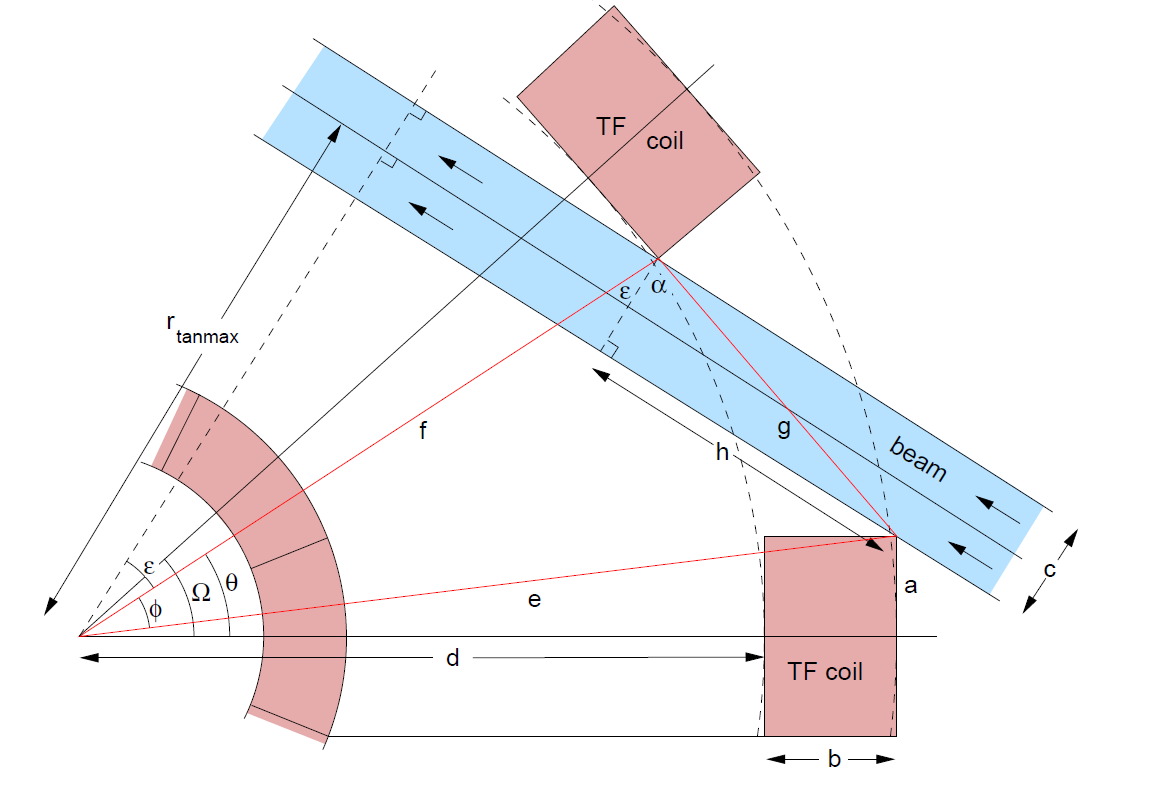
\includegraphics[scale=0.4]{archive/figures/beam_access.PNG}
    \caption{PROCESS beam access layout.} \label{fig: beam-access}
    \end{figure}

    \begin{equation}\label{eq: beam-a-omega}
        \Omega = \frac{2\pi}{N_{TF}}
    \end{equation}

    \begin{equation}\label{eq: beam-a-f}
        F = \sqrt{(\frac{h}{2})^2) + (L + b)^2 }
    \end{equation}

    \begin{equation}\label{eq: beam-a-h}
        H = \sqrt{ L^2 - (\frac{h}{2})^2 }
    \end{equation}

    \begin{equation}\label{eq: beam-a-theta}
        \theta = \Omega - \tan^{-1} \left ( \frac{h/2}{L} \right)
    \end{equation}

    \begin{equation}\label{eq: beam-a-phi}
        \phi = \theta - \tan^{-1} \left ( \frac{h/2}{L + b}  \right )
    \end{equation}

    \begin{equation}\label{eq: beam-a-g}
        G = \sqrt{H^2 + F^2 -2HF\cos \phi}
    \end{equation}

    \noi $N_{TF}$ is the number of TF coils, and $C$ is the width required for 
    the neutral beam duct, including any shielding required to protect the TF 
    coils on either side, the thickness of the duct wall, the thermal shields 
    and the vacuum gaps.

    \begin{equation}\label{eq: beam-a-j}
        J = \sqrt{G^2 - C^2}
    \end{equation}

    \begin{equation}\label{eq: beam-a-epsilon}
        \epsilon = \sin^{-1} \left ( \frac{F\sin \phi}{G} \right ) - 
        \tan^{-1} \left ( \frac{J}{C} \right )
    \end{equation}

    \noi The maximum possible tangency radius is

    \begin{equation}\label{eq: beam-a-rtan}
        R_{tanmax} = H \cos(\epsilon) - \frac{C}{2}
    \end{equation}

    \bibliography{tf_refs.bib}{}
    \bibliographystyle{plain}
    
    \end{document}
    